\documentclass[a4paper, 11pt]{article}
\usepackage[portuguese]{babel}
\usepackage{graphicx} % Required for inserting images
\usepackage{xcolor} % For syntax highlighting colors


\title{Teste Modelo de Sistemas Operativos}
\author{Eduardo Fernandes}
\date{2024/2025}

\begin{document}

\maketitle


\section*{Questões Teóricas}

\noindent \textbf{Questão 1}\\

\noindent O escalonador de processos procura manter uma mistura equilibrada de processos intensivos em CPU e em I/O porque isso permite uma utilização mais eficiente dos recursos do sistema. Enquanto processos intensivos em I/O aguardam a conclusão de operações em dispositivos externos, o CPU pode ser utilizado por processos que requerem muita computação. Isto permite estabelecer paralelismo entre processos, maximizando a utilização dos recursos do sistema. Este paralelismo permite aumentar o desempenho do sistema, pois temos mais processos a executar concorrentemente.\\


\noindent \textbf{Questão 2}\\

\noindent Para o sistema operativo apresentado, escolheria o algoritmo de escalonamento \textbf{MLFQ} (Multi Level Feedback Queue). Este algoritmo distribui a execução de processos em filas de espera com prioridade, sendo a primeira fila a que tem maior prioridade. A cada processo é atribuída uma porção de tempo em cada fila, e periodicamente cada processo é elevado para a fila de cima.\\

\noindent Uma das \textbf{vantagens} deste algoritmo é o baixo turn around time e response time, pois processos rápidos com baixa duração executam rapidamente e processos com alta prioridade são frequentemente trocados, aproximando-se do algoritmo Round Robin. Uma \textbf{preocupação} para este algoritmo é determinar o número de filas de espera, a porção de tempo para cada processo em cada fila e quando cada processo deve ser elevado, pois é necessário efetuar uma configuração cuidadosa e saber estatísticas relativas à utilização do sistema.

\newpage

\noindent \textbf{Questão 3}

\begin{enumerate}
    \item Combinar paginação com mecanismos de swapping é uma técnica muito \textbf{vantajosa}, pois permite aos programadores desenvolver programas, sem se preocupar com o facto de as suas estruturas de dados cabem ou não na memória fisica, isto é, permite ter programas que ocupam um espaço maior que a própria memória principal. Uma \textbf{preocupação} que o sistema operativo deve ter é a substituição de páginas quando a área de swap está cheia. Se o sistema operativo remover páginas que são frequentemente usadas, perde eficiencia (muitos acessos a disco), logo é necessário ter uma boa política de substituição para minimizar page faults.
    
    \item É preferivel usar uma \textbf{partição de disco}, pois evita a sobrecarga associada à gestão do sistema de ficheiros (alocação de blocos, verificação de permissões, ...) tornando o acesso à swap mais rápido e eficiente.
\end{enumerate}

\noindent \textbf{Questão 4}\\

\noindent Uma possível razão para o mau desempenho das aplicações é o facto de os pedidos que se situam mais longe dos cilindros não chegarem a ser realizados, caso sejam feitos pedidos que estejam mais próximos da cabeça do disco, que têm maior prioridade. Um algoritmo de escalonamento capaz de melhorar a desempenho destas aplicações é o algoritmo \textbf{Circular SCAN}, que percorre o disco, da track mais exterior para a mais interior e vice-versa. Este algoritmo de elevador é justo para qualquer pedido a qualquer track.\\

\noindent \textbf{Questão 5}\\

\noindent \fbox{B} Shortest Job First (SJF).\\

\noindent \fbox{C} First-Come First-Served (FCFS).\\

\noindent \textbf{Questão 6}\\

\noindent \fbox{D} A paginação de memória pode gerar fragmentação interna mas não externa.\\

\noindent \textbf{Questão 7}\\

\noindent \fbox{B} Sim, tempos de acesso aleatório são mais altos do que tempos de acesso sequenciais em discos HDD.\\

\noindent \fbox{D} Sim, já que tende a diminuir o tempo médio de seek do disco HDD.

\newpage

\section*{Questões Práticas}

\noindent \textbf{Questão 8}\\

\noindent Resolução apresentada no ficheiro \fbox{\texttt{question-8.c}}\\


\noindent \textbf{Questão 9}\\

\noindent Resolução apresentada no ficheiro \fbox{\texttt{question-9.c}}\\


\noindent \textbf{Questão 10}\\

\noindent Resolução apresentada nos ficheiros \fbox{\texttt{SOGPT.c}} e \fbox{\texttt{servidor.c}}

\begin{figure}[h]
    \centering
    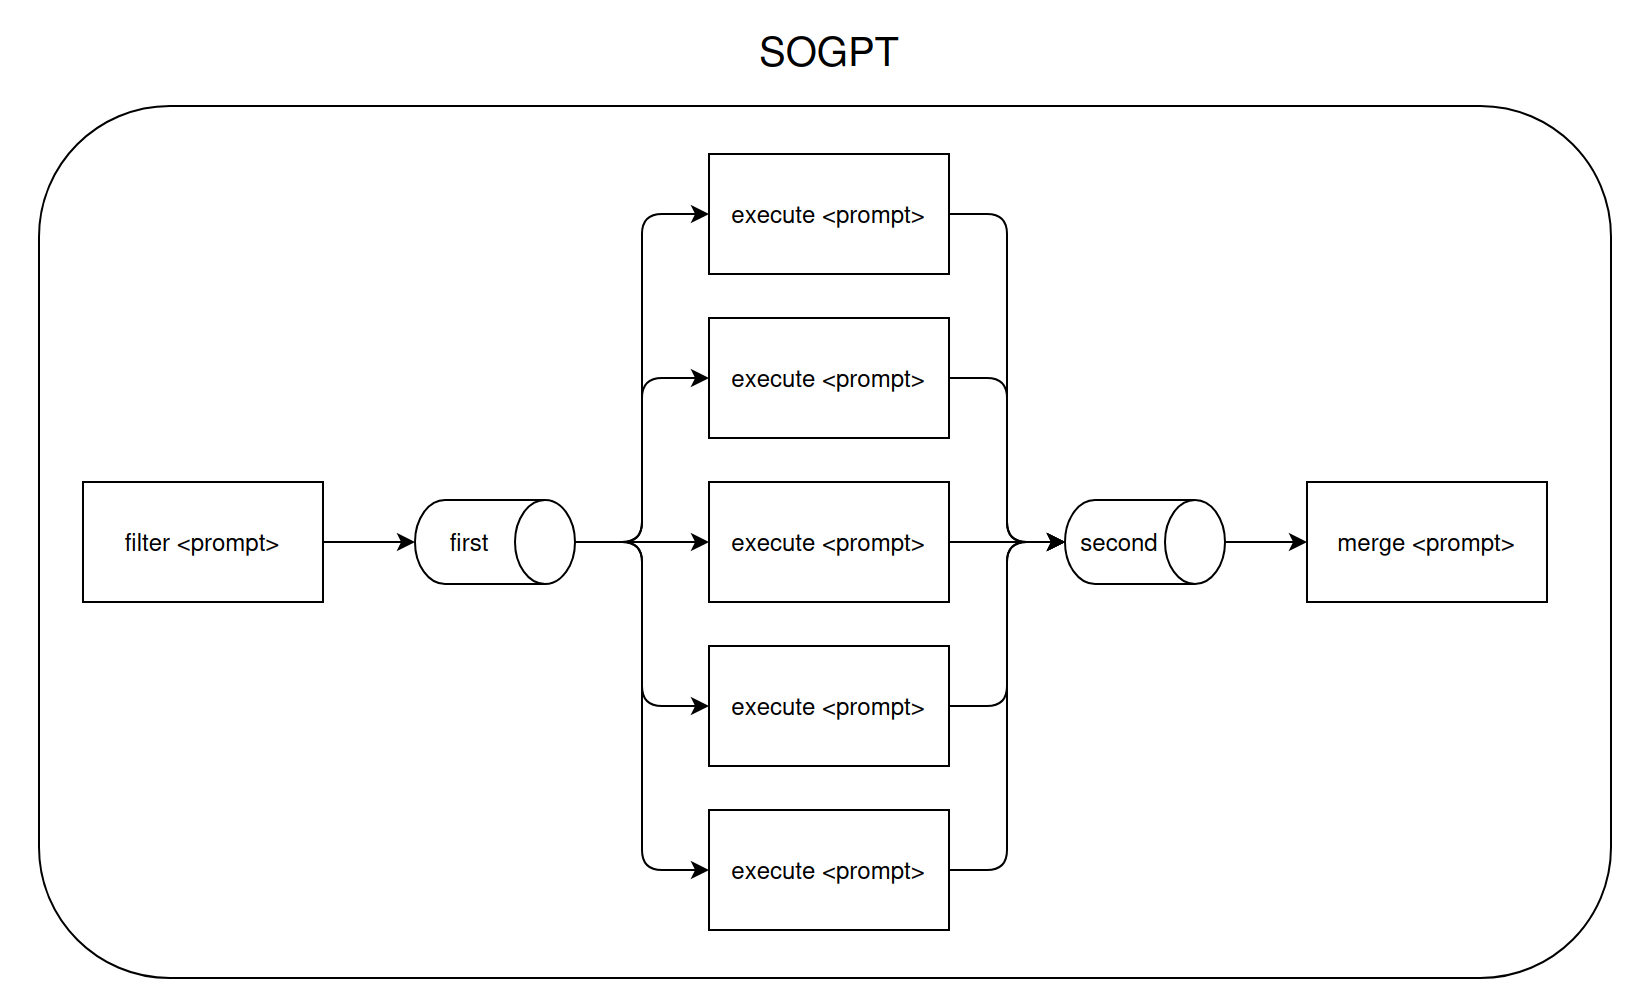
\includegraphics[width=1\linewidth]{questao-10-diagrama.png}
    \caption{Diagrama SOGPT}
\end{figure}

\noindent Se a abertura do pipe com nome \texttt{fifoc\_name} (linha 15) fosse feita logo após a criação do mesmo (linha 8), o programa não iria funcionar devido ao facto de o cliente bloquear na abertura do pipe \texttt{fifoc\_name}, que consequentemente iria bloquear o servidor na abertura do pipe \texttt{fifo\_server}, pois todos os clientes ficam bloqueados no \texttt{open("fifoc\_name", O\_WRONLY)}. Por outras palavras, o programa \texttt{cliente} iria bloquear na abertura do pipe com nome \texttt{fifoc\_name}, e como o servidor apenas abre esse canal após a abertura do pipe \texttt{fifo\_server}, este fica bloqueado, pois todos os clientes abrem o canal \texttt{fifo\_server} após a abertura do \texttt{fifoc\_name}.\\

\newpage

\noindent \textbf{Questão 11}\\

\noindent \fbox{C} A operação \texttt{op(...)} no máximo executa 10 vezes.\\


\noindent \textbf{Questão 12}\\

\noindent \fbox{A} O programa cria processos que executam a \texttt{func1()} sequencialmente.\\

\noindent \fbox{D} O output esperado é:
\begin{verbatim}
        processo 0
        processo 0 terminou
        processo 1
        processo 1 terminou
        processo 2
        processo 2 terminou
\end{verbatim}


\noindent \textbf{Questão 13}\\

\noindent \fbox{C} \texttt{lseek(fd, sizeof(Matricula) * 11, SEEK\_SET);}\\


\noindent \textbf{Questão 14}\\

\noindent \fbox{A} Após um cliente terminar a sua execução, e caso não exista mais nenhum cliente a executar, o servidor termina também o seu programa e não atende mais clientes.\\

\noindent \fbox{D} Após um cliente terminar a sua execução, caso estejam outros programas clientes a enviar mensagens para o servidor, o servidor continua a executar o seu programa e a atender outros clientes até que todos tenham terminado.\\


\noindent \textbf{Questão 15}\\

\noindent \fbox{B} O seguinte código está em falta (linha 25)
\begin{verbatim}
        1   close(pfd[0][0]);
        2   close(pfd[1][1]);
\end{verbatim}

\noindent \fbox{D} O programa emula o comando \texttt{cat etc/passwd | sort | wc -l}


\end{document}
